\chapter{The House of Morrel \& Son}

Anyone who had quitted Marseilles a few years previously, well
acquainted with the interior of Morrel’s warehouse, and had returned at
this date, would have found a great change. Instead of that air of
life, of comfort, and of happiness that permeates a flourishing and
prosperous business establishment—instead of merry faces at the
windows, busy clerks hurrying to and fro in the long corridors—instead
of the court filled with bales of goods, re-echoing with the cries and
the jokes of porters, one would have immediately perceived all aspect
of sadness and gloom. Out of all the numerous clerks that used to fill
the deserted corridor and the empty office, but two remained. One was a
young man of three or four-and-twenty, who was in love with M. Morrel’s
daughter, and had remained with him in spite of the efforts of his
friends to induce him to withdraw; the other was an old one-eyed
cashier, called “Cocles,” or “Cock-eye,” a nickname given him by the
young men who used to throng this vast now almost deserted bee-hive,
and which had so completely replaced his real name that he would not,
in all probability, have replied to anyone who addressed him by it.

Cocles remained in M. Morrel’s service, and a most singular change had
taken place in his position; he had at the same time risen to the rank
of cashier, and sunk to the rank of a servant. He was, however, the
same Cocles, good, patient, devoted, but inflexible on the subject of
arithmetic, the only point on which he would have stood firm against
the world, even against M. Morrel; and strong in the
multiplication-table, which he had at his fingers’ ends, no matter what
scheme or what trap was laid to catch him.

In the midst of the disasters that befell the house, Cocles was the
only one unmoved. But this did not arise from a want of affection; on
the contrary, from a firm conviction. Like the rats that one by one
forsake the doomed ship even before the vessel weighs anchor, so all
the numerous clerks had by degrees deserted the office and the
warehouse. Cocles had seen them go without thinking of inquiring the
cause of their departure. Everything was as we have said, a question of
arithmetic to Cocles, and during twenty years he had always seen all
payments made with such exactitude, that it seemed as impossible to him
that the house should stop payment, as it would to a miller that the
river that had so long turned his mill should cease to flow.

Nothing had as yet occurred to shake Cocles’ belief; the last month’s
payment had been made with the most scrupulous exactitude; Cocles had
detected an overbalance of fourteen sous in his cash, and the same
evening he had brought them to M. Morrel, who, with a melancholy smile,
threw them into an almost empty drawer, saying:

“Thanks, Cocles; you are the pearl of cashiers.”

Cocles went away perfectly happy, for this eulogium of M. Morrel,
himself the pearl of the honest men of Marseilles, flattered him more
than a present of fifty crowns. But since the end of the month M.
Morrel had passed many an anxious hour.

In order to meet the payments then due; he had collected all his
resources, and, fearing lest the report of his distress should get
bruited abroad at Marseilles when he was known to be reduced to such an
extremity, he went to the Beaucaire fair to sell his wife’s and
daughter’s jewels and a portion of his plate. By this means the end of
the month was passed, but his resources were now exhausted. Credit,
owing to the reports afloat, was no longer to be had; and to meet the
one hundred thousand francs due on the 15th of the present month, and
the one hundred thousand francs due on the 15th of the next month to M.
de Boville, M. Morrel had, in reality, no hope but the return of the
\textit{Pharaon}, of whose departure he had learnt from a vessel which had
weighed anchor at the same time, and which had already arrived in
harbor.

But this vessel which, like the \textit{Pharaon}, came from Calcutta, had been
in for a fortnight, while no intelligence had been received of the
\textit{Pharaon}.

\begin{figure}[ht]
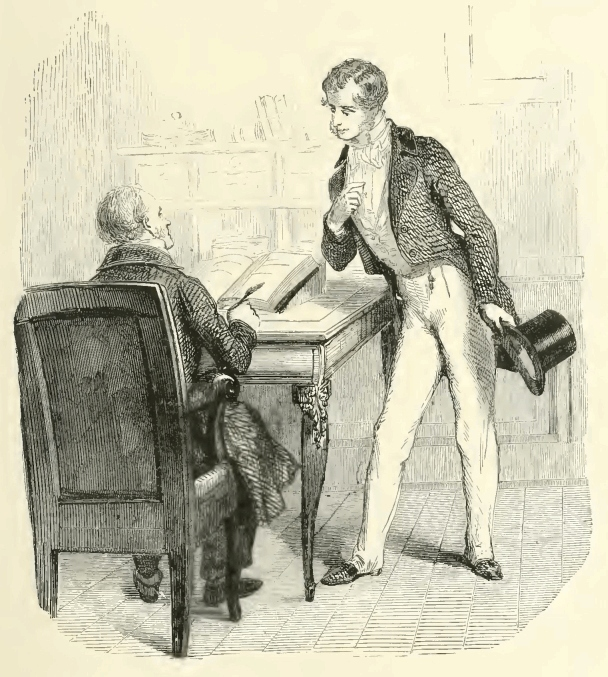
\includegraphics[width=\textwidth]{20033m.jpg}
\end{figure}

Such was the state of affairs when, the day after his interview with M.
de Boville, the confidential clerk of the house of Thomson \& French of
Rome, presented himself at M. Morrel’s.

Emmanuel received him; this young man was alarmed by the appearance of
every new face, for every new face might be that of a new creditor,
come in anxiety to question the head of the house. The young man,
wishing to spare his employer the pain of this interview, questioned
the new-comer; but the stranger declared that he had nothing to say to
M. Emmanuel, and that his business was with M. Morrel in person.

Emmanuel sighed, and summoned Cocles. Cocles appeared, and the young
man bade him conduct the stranger to M. Morrel’s apartment. Cocles went
first, and the stranger followed him. On the staircase they met a
beautiful girl of sixteen or seventeen, who looked with anxiety at the
stranger.

“M. Morrel is in his room, is he not, Mademoiselle Julie?” said the
cashier.

“Yes; I think so, at least,” said the young girl hesitatingly. “Go and
see, Cocles, and if my father is there, announce this gentleman.”

“It will be useless to announce me, mademoiselle,” returned the
Englishman. “M. Morrel does not know my name; this worthy gentleman has
only to announce the confidential clerk of the house of Thomson \&
French of Rome, with whom your father does business.”

The young girl turned pale and continued to descend, while the stranger
and Cocles continued to mount the staircase. She entered the office
where Emmanuel was, while Cocles, by the aid of a key he possessed,
opened a door in the corner of a landing-place on the second staircase,
conducted the stranger into an antechamber, opened a second door, which
he closed behind him, and after having left the clerk of the house of
Thomson \& French alone, returned and signed to him that he could enter.

The Englishman entered, and found Morrel seated at a table, turning
over the formidable columns of his ledger, which contained the list of
his liabilities. At the sight of the stranger, M. Morrel closed the
ledger, arose, and offered a seat to the stranger; and when he had seen
him seated, resumed his own chair. Fourteen years had changed the
worthy merchant, who, in his thirty-sixth year at the opening of this
history, was now in his fiftieth; his hair had turned white, time and
sorrow had ploughed deep furrows on his brow, and his look, once so
firm and penetrating, was now irresolute and wandering, as if he feared
being forced to fix his attention on some particular thought or person.

The Englishman looked at him with an air of curiosity, evidently
mingled with interest. “Monsieur,” said Morrel, whose uneasiness was
increased by this examination, “you wish to speak to me?”

“Yes, monsieur; you are aware from whom I come?”

“The house of Thomson \& French; at least, so my cashier tells me.”

“He has told you rightly. The house of Thomson \& French had 300,000 or
400,000 francs to pay this month in France; and, knowing your strict
punctuality, have collected all the bills bearing your signature, and
charged me as they became due to present them, and to employ the money
otherwise.”

Morrel sighed deeply, and passed his hand over his forehead, which was
covered with perspiration.

“So then, sir,” said Morrel, “you hold bills of mine?”

“Yes, and for a considerable sum.”

“What is the amount?” asked Morrel with a voice he strove to render
firm.

\begin{figure}[ht]
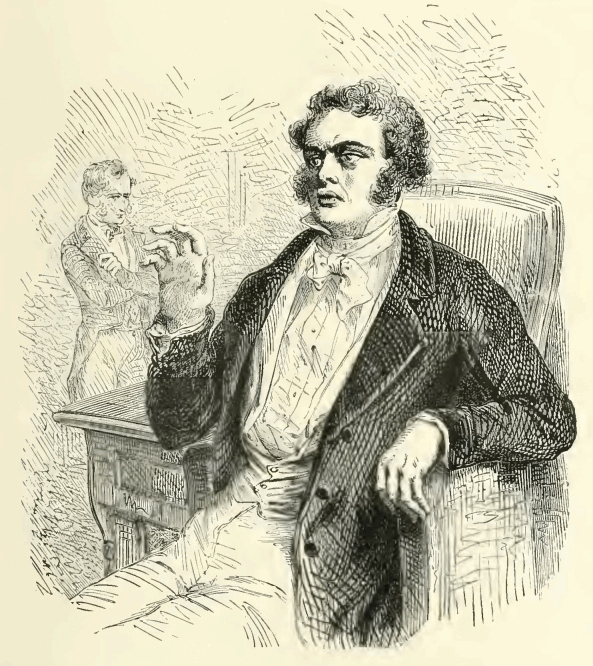
\includegraphics[width=\textwidth]{20035m.jpg}
\end{figure}

“Here is,” said the Englishman, taking a quantity of papers from his
pocket, “an assignment of 200,000 francs to our house by M. de Boville,
the inspector of prisons, to whom they are due. You acknowledge, of
course, that you owe this sum to him?”

“Yes; he placed the money in my hands at four and a half per cent
nearly five years ago.”

“When are you to pay?”

“Half the 15th of this month, half the 15th of next.”

“Just so; and now here are 32,500 francs payable shortly; they are all
signed by you, and assigned to our house by the holders.”

“I recognize them,” said Morrel, whose face was suffused, as he thought
that, for the first time in his life, he would be unable to honor his
own signature. “Is this all?”

“No, I have for the end of the month these bills which have been
assigned to us by the house of Pascal, and the house of Wild \& Turner
of Marseilles, amounting to nearly 55,000 francs; in all, 287,500
francs.”

It is impossible to describe what Morrel suffered during this
enumeration. “Two hundred and eighty-seven thousand five hundred
francs,” repeated he.

“Yes, sir,” replied the Englishman. “I will not,” continued he, after a
moment’s silence, “conceal from you, that while your probity and
exactitude up to this moment are universally acknowledged, yet the
report is current in Marseilles that you are not able to meet your
liabilities.”

At this almost brutal speech Morrel turned deathly pale.

“Sir,” said he, “up to this time—and it is now more than
four-and-twenty years since I received the direction of this house from
my father, who had himself conducted it for five-and-thirty years—never
has anything bearing the signature of Morrel \& Son been dishonored.”

“I know that,” replied the Englishman. “But as a man of honor should
answer another, tell me fairly, shall you pay these with the same
punctuality?”

Morrel shuddered, and looked at the man, who spoke with more assurance
than he had hitherto shown.

“To questions frankly put,” said he, “a straightforward answer should
be given. Yes, I shall pay, if, as I hope, my vessel arrives safely;
for its arrival will again procure me the credit which the numerous
accidents, of which I have been the victim, have deprived me; but if
the \textit{Pharaon} should be lost, and this last resource be gone——”

The poor man’s eyes filled with tears.

“Well,” said the other, “if this last resource fail you?”

“Well,” returned Morrel, “it is a cruel thing to be forced to say, but,
already used to misfortune, I must habituate myself to shame. I fear I
shall be forced to suspend payment.”

“Have you no friends who could assist you?”

Morrel smiled mournfully.

“In business, sir,” said he, “one has no friends, only correspondents.”

“It is true,” murmured the Englishman; “then you have but one hope.”

“But one.”

“The last?”

“The last.”

“So that if this fail——”

“I am ruined,—completely ruined!”

“As I was on my way here, a vessel was coming into port.”

“I know it, sir; a young man, who still adheres to my fallen fortunes,
passes a part of his time in a belvedere at the top of the house, in
hopes of being the first to announce good news to me; he has informed
me of the arrival of this ship.”

“And it is not yours?”

“No, she is a Bordeaux vessel, \textit{La Gironde}; she comes from India also;
but she is not mine.”

“Perhaps she has spoken to the \textit{Pharaon}, and brings you some tidings
of her?”

“Shall I tell you plainly one thing, sir? I dread almost as much to
receive any tidings of my vessel as to remain in doubt. Uncertainty is
still hope.” Then in a low voice Morrel added,—“This delay is not
natural. The \textit{Pharaon} left Calcutta the 5th of February; she ought to
have been here a month ago.”

“What is that?” said the Englishman. “What is the meaning of that
noise?”

“Oh, my God!” cried Morrel, turning pale, “what is it?”

A loud noise was heard on the stairs of people moving hastily, and
half-stifled sobs. Morrel rose and advanced to the door; but his
strength failed him and he sank into a chair. The two men remained
opposite one another, Morrel trembling in every limb, the stranger
gazing at him with an air of profound pity. The noise had ceased; but
it seemed that Morrel expected something—something had occasioned the
noise, and something must follow. The stranger fancied he heard
footsteps on the stairs; and that the footsteps, which were those of
several persons, stopped at the door. A key was inserted in the lock of
the first door, and the creaking of hinges was audible.

“There are only two persons who have the key to that door,” murmured
Morrel, “Cocles and Julie.”

At this instant the second door opened, and the young girl, her eyes
bathed with tears, appeared. Morrel rose tremblingly, supporting
himself by the arm of the chair. He would have spoken, but his voice
failed him.

“Oh, father!” said she, clasping her hands, “forgive your child for
being the bearer of evil tidings.”

Morrel again changed color. Julie threw herself into his arms.

“Oh, father, father!” murmured she, “courage!”

“The \textit{Pharaon} has gone down, then?” said Morrel in a hoarse voice. The
young girl did not speak; but she made an affirmative sign with her
head as she lay on her father’s breast.

“And the crew?” asked Morrel.

“Saved,” said the girl; “saved by the crew of the vessel that has just
entered the harbor.”

Morrel raised his two hands to heaven with an expression of resignation
and sublime gratitude.

“Thanks, my God,” said he, “at least thou strikest but me alone.”

A tear moistened the eye of the phlegmatic Englishman.

“Come in, come in,” said Morrel, “for I presume you are all at the
door.”

Scarcely had he uttered those words when Madame Morrel entered weeping
bitterly. Emmanuel followed her, and in the antechamber were visible
the rough faces of seven or eight half-naked sailors. At the sight of
these men the Englishman started and advanced a step; then restrained
himself, and retired into the farthest and most obscure corner of the
apartment. Madame Morrel sat down by her husband and took one of his
hands in hers, Julie still lay with her head on his shoulder, Emmanuel
stood in the centre of the chamber and seemed to form the link between
Morrel’s family and the sailors at the door.

“How did this happen?” said Morrel.

“Draw nearer, Penelon,” said the young man, “and tell us all about it.”

An old seaman, bronzed by the tropical sun, advanced, twirling the
remains of a hat between his hands.

“Good-day, M. Morrel,” said he, as if he had just quitted Marseilles
the previous evening, and had just returned from Aix or Toulon.

“Good-day, Penelon,” returned Morrel, who could not refrain from
smiling through his tears, “where is the captain?”

“The captain, M. Morrel,—he has stayed behind sick at Palma; but please
God, it won’t be much, and you will see him in a few days all alive and
hearty.”

“Well, now tell your story, Penelon.”

\begin{figure}[ht]
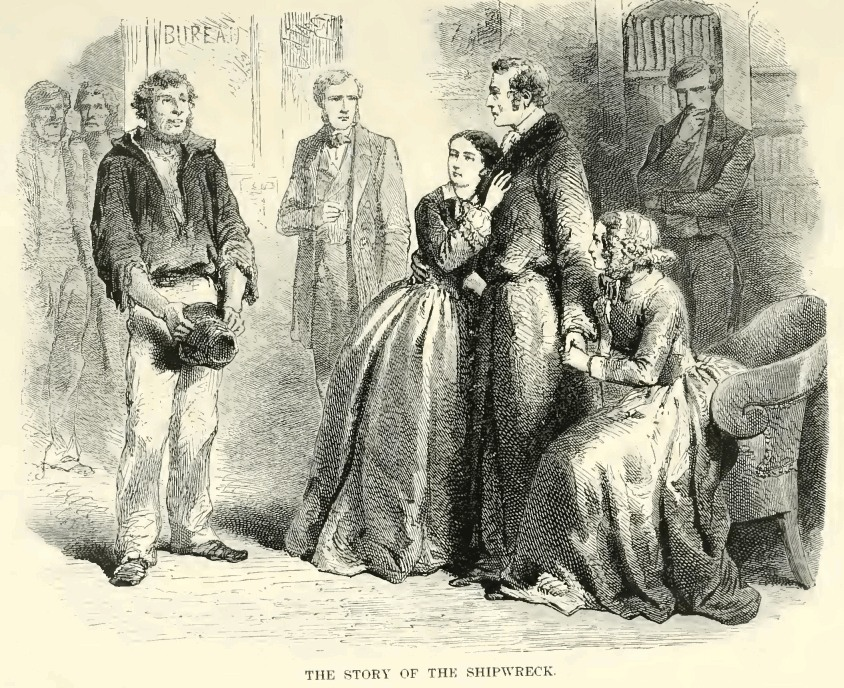
\includegraphics[width=\textwidth]{20039m.jpg}
\end{figure}

Penelon rolled his quid in his cheek, placed his hand before his mouth,
turned his head, and sent a long jet of tobacco-juice into the
antechamber, advanced his foot, balanced himself, and began.

“You see, M. Morrel,” said he, “we were somewhere between Cape Blanc
and Cape Boyador, sailing with a fair breeze, south-south-west after a
week’s calm, when Captain Gaumard comes up to me—I was at the helm I
should tell you—and says, ‘Penelon, what do you think of those clouds
coming up over there?’ I was just then looking at them myself. ‘What do
I think, captain? Why I think that they are rising faster than they
have any business to do, and that they would not be so black if they
didn’t mean mischief.’—‘That’s my opinion too,’ said the captain, ‘and
I’ll take precautions accordingly. We are carrying too much canvas.
Avast, there, all hands! Take in the studding-sails and stow the flying
jib.’ It was time; the squall was on us, and the vessel began to heel.
‘Ah,’ said the captain, ‘we have still too much canvas set; all hands
lower the mainsail!’ Five minutes after, it was down; and we sailed
under mizzen-topsails and top-gallant sails. ‘Well, Penelon,’ said the
captain, ‘what makes you shake your head?’ ‘Why,’ I says, ‘I still
think you’ve got too much on.’ ‘I think you’re right,’ answered he, ‘we
shall have a gale.’ ‘A gale? More than that, we shall have a tempest,
or I don’t know what’s what.’ You could see the wind coming like the
dust at Montredon; luckily the captain understood his business. ‘Take
in two reefs in the top-sails,’ cried the captain; ‘let go the
bowlin’s, haul the brace, lower the top-gallant sails, haul out the
reef-tackles on the yards.’”

\begin{figure}[ht]
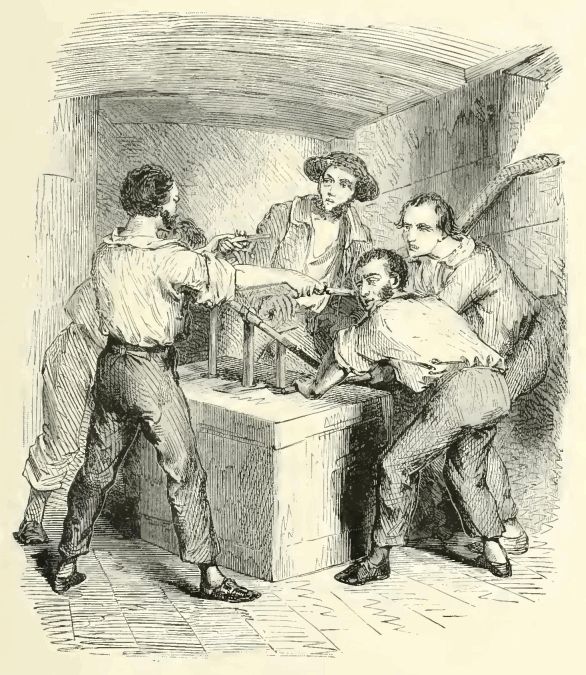
\includegraphics[width=\textwidth]{20041m.jpg}
\end{figure}

“That was not enough for those latitudes,” said the Englishman; “I
should have taken four reefs in the topsails and furled the spanker.”

His firm, sonorous, and unexpected voice made everyone start. Penelon
put his hand over his eyes, and then stared at the man who thus
criticized the manœuvres of his captain.

“We did better than that, sir,” said the old sailor respectfully; “we
put the helm up to run before the tempest; ten minutes after we struck
our top-sails and scudded under bare poles.”

“The vessel was very old to risk that,” said the Englishman.

“Eh, it was that that did the business; after pitching heavily for
twelve hours we sprung a leak. ‘Penelon,’ said the captain, ‘I think we
are sinking, give me the helm, and go down into the hold.’ I gave him
the helm, and descended; there was already three feet of water. ‘All
hands to the pumps!’ I shouted; but it was too late, and it seemed the
more we pumped the more came in. ‘Ah,’ said I, after four hours’ work,
‘since we are sinking, let us sink; we can die but once.’ ‘Is that the
example you set, Penelon?’ cries the captain; ‘very well, wait a
minute.’ He went into his cabin and came back with a brace of pistols.
‘I will blow the brains out of the first man who leaves the pump,’ said
he.”

“Well done!” said the Englishman.

\begin{figure}[ht]
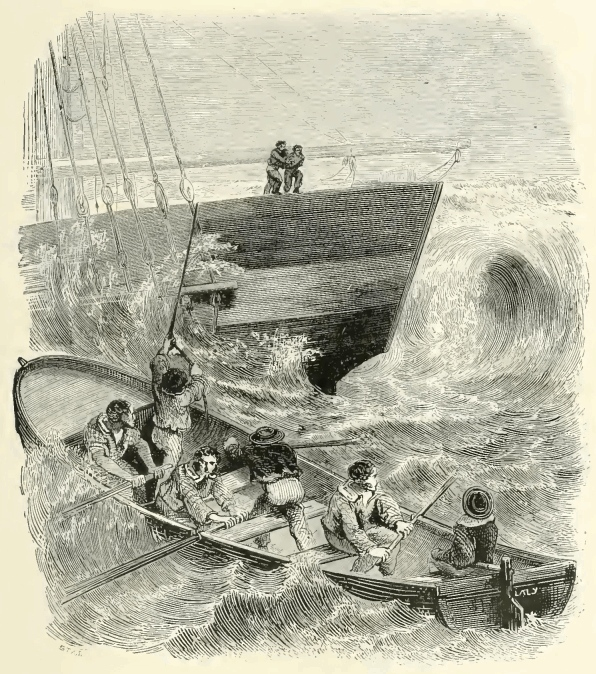
\includegraphics[width=\textwidth]{20043m.jpg}
\end{figure}

“There’s nothing gives you so much courage as good reasons,” continued
the sailor; “and during that time the wind had abated, and the sea gone
down, but the water kept rising; not much, only two inches an hour, but
still it rose. Two inches an hour does not seem much, but in twelve
hours that makes two feet, and three we had before, that makes five.
‘Come,’ said the captain, ‘we have done all in our power, and M. Morrel
will have nothing to reproach us with, we have tried to save the ship,
let us now save ourselves. To the boats, my lads, as quick as you can.’
Now,” continued Penelon, “you see, M. Morrel, a sailor is attached to
his ship, but still more to his life, so we did not wait to be told
twice; the more so, that the ship was sinking under us, and seemed to
say, ‘Get along—save yourselves.’ We soon launched the boat, and all
eight of us got into it. The captain descended last, or rather, he did
not descend, he would not quit the vessel; so I took him round the
waist, and threw him into the boat, and then I jumped after him. It was
time, for just as I jumped the deck burst with a noise like the
broadside of a man-of-war. Ten minutes after she pitched forward, then
the other way, spun round and round, and then good-bye to the
\textit{Pharaon}. As for us, we were three days without anything to eat or
drink, so that we began to think of drawing lots who should feed the
rest, when we saw \textit{La Gironde}; we made signals of distress, she
perceived us, made for us, and took us all on board. There now, M.
Morrel, that’s the whole truth, on the honor of a sailor; is not it
true, you fellows there?” A general murmur of approbation showed that
the narrator had faithfully detailed their misfortunes and sufferings.

“Well, well,” said M. Morrel, “I know there was no one in fault but
destiny. It was the will of God that this should happen, blessed be his
name. What wages are due to you?”

“Oh, don’t let us talk of that, M. Morrel.”

“Yes, but we will talk of it.”

“Well, then, three months,” said Penelon.

“Cocles, pay two hundred francs to each of these good fellows,” said
Morrel. “At another time,” added he, “I should have said, Give them,
besides, two hundred francs over as a present; but times are changed,
and the little money that remains to me is not my own, so do not think
me mean on this account.”

Penelon turned to his companions, and exchanged a few words with them.

“As for that, M. Morrel,” said he, again turning his quid, “as for
that——”

“As for what?”

“The money.”

“Well——”

“Well, we all say that fifty francs will be enough for us at present,
and that we will wait for the rest.”

“Thanks, my friends, thanks!” cried Morrel gratefully; “take it—take
it; and if you can find another employer, enter his service; you are
free to do so.”

These last words produced a prodigious effect on the seaman. Penelon
nearly swallowed his quid; fortunately he recovered.

“What, M. Morrel!” said he in a low voice, “you send us away; you are
then angry with us!”

“No, no,” said M. Morrel, “I am not angry, quite the contrary, and I do
not send you away; but I have no more ships, and therefore I do not
want any sailors.”

“No more ships!” returned Penelon; “well, then, you’ll build some;
we’ll wait for you.”

“I have no money to build ships with, Penelon,” said the poor owner
mournfully, “so I cannot accept your kind offer.”

“No more money? Then you must not pay us; we can scud, like the
\textit{Pharaon}, under bare poles.”

“Enough, enough!” cried Morrel, almost overpowered; “leave me, I pray
you; we shall meet again in a happier time. Emmanuel, go with them, and
see that my orders are executed.”

“At least, we shall see each other again, M. Morrel?” asked Penelon.

“Yes; I hope so, at least. Now go.” He made a sign to Cocles, who went
first; the seamen followed him and Emmanuel brought up the rear. “Now,”
said the owner to his wife and daughter, “leave me; I wish to speak
with this gentleman.”

\begin{figure}[ht]
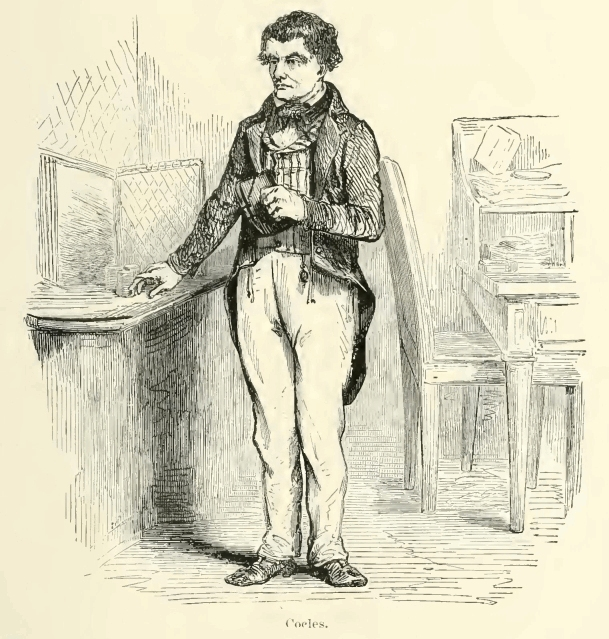
\includegraphics[width=\textwidth]{20045m.jpg}
\end{figure}

And he glanced towards the clerk of Thomson \& French, who had remained
motionless in the corner during this scene, in which he had taken no
part, except the few words we have mentioned. The two women looked at
this person whose presence they had entirely forgotten, and retired;
but, as she left the apartment, Julie gave the stranger a supplicating
glance, to which he replied by a smile that an indifferent spectator
would have been surprised to see on his stern features. The two men
were left alone. “Well, sir,” said Morrel, sinking into a chair, “you
have heard all, and I have nothing further to tell you.”

“I see,” returned the Englishman, “that a fresh and unmerited
misfortune has overwhelmed you, and this only increases my desire to
serve you.”

“Oh, sir!” cried Morrel.

“Let me see,” continued the stranger, “I am one of your largest
creditors.”

“Your bills, at least, are the first that will fall due.”

“Do you wish for time to pay?”

“A delay would save my honor, and consequently my life.”

“How long a delay do you wish for?”

Morrel reflected. “Two months,” said he.

“I will give you three,” replied the stranger.

“But,” asked Morrel, “will the house of Thomson \& French consent?”

“Oh, I take everything on myself. Today is the 5th of June.”

“Yes.”

“Well, renew these bills up to the 5th of September; and on the 5th of
September at eleven o’clock (the hand of the clock pointed to eleven),
I shall come to receive the money.”

“I shall expect you,” returned Morrel; “and I will pay you—or I shall
be dead.” These last words were uttered in so low a tone that the
stranger could not hear them. The bills were renewed, the old ones
destroyed, and the poor ship-owner found himself with three months
before him to collect his resources. The Englishman received his thanks
with the phlegm peculiar to his nation; and Morrel, overwhelming him
with grateful blessings, conducted him to the staircase. The stranger
met Julie on the stairs; she pretended to be descending, but in reality
she was waiting for him. “Oh, sir”—said she, clasping her hands.

“Mademoiselle,” said the stranger, “one day you will receive a letter
signed ‘Sinbad the Sailor.’ Do exactly what the letter bids you,
however strange it may appear.”

“Yes, sir,” returned Julie.

“Do you promise?”

“I swear to you I will.”

“It is well. Adieu, mademoiselle. Continue to be the good, sweet girl
you are at present, and I have great hopes that Heaven will reward you
by giving you Emmanuel for a husband.”

Julie uttered a faint cry, blushed like a rose, and leaned against the
baluster. The stranger waved his hand, and continued to descend. In the
court he found Penelon, who, with a rouleau of a hundred francs in
either hand, seemed unable to make up his mind to retain them. “Come
with me, my friend,” said the Englishman; “I wish to speak to you.”
